\subsection{More Questions}
Possible things that maybe beneficial to look at, table \ref{tab:open_issues}.
\begin{table*}
\centering
\begin{tabular}{l|l}
Issue & difficulty/impact \\\hline
Huge pages in \oursys & Few days of work expected <+5\% improved performance \\
New Theory: Add triger to NAPI call with TX Ring watermarks? & Awsome for TX and should also work for TCP\\
ad hoc NAPI budget & minor but could be interesting\\
TCP flows & why more than one flow needed to saturate single core?\\
Is prefetch usefull&\\
Inline functions & a known issue in the Linux community\\
UDP fragment losses & Not sure there is a resolution in SW\\
lock in TX queue & if were dealing with locks already...\\
coalescing & with higher rates may be its time to revisit?\\
Is xmit more used? & batching in send, could show up to +5\%\\
ad hoc driver memory reuse & motivation?\\
PFC & PFC has an impact on TCP performance, never looked at why\\
\hline
\end{tabular}
\caption{\label{tab:open_issues}Open issues}
\end{table*}

\subsection{Memory allocator}
The Linux memory allocator, is an all purpose allocator that must cater to a multitude of scenarios. The allocator needs to deal with issues like;
\begin{itemize}
    \item Fragmentation
    \item Page migration (user-space migrating to other NODE)
    \item Zones 
    \item recursive allocations (alloc code that needs to alloc code)
    \item variable sizes
\end{itemize}

The hierarchy of data structures associated with a zoned memory allocator are shown in figure \ref{fig:zoned_memory_alloc}.
\begin{figure*}
    \centering
    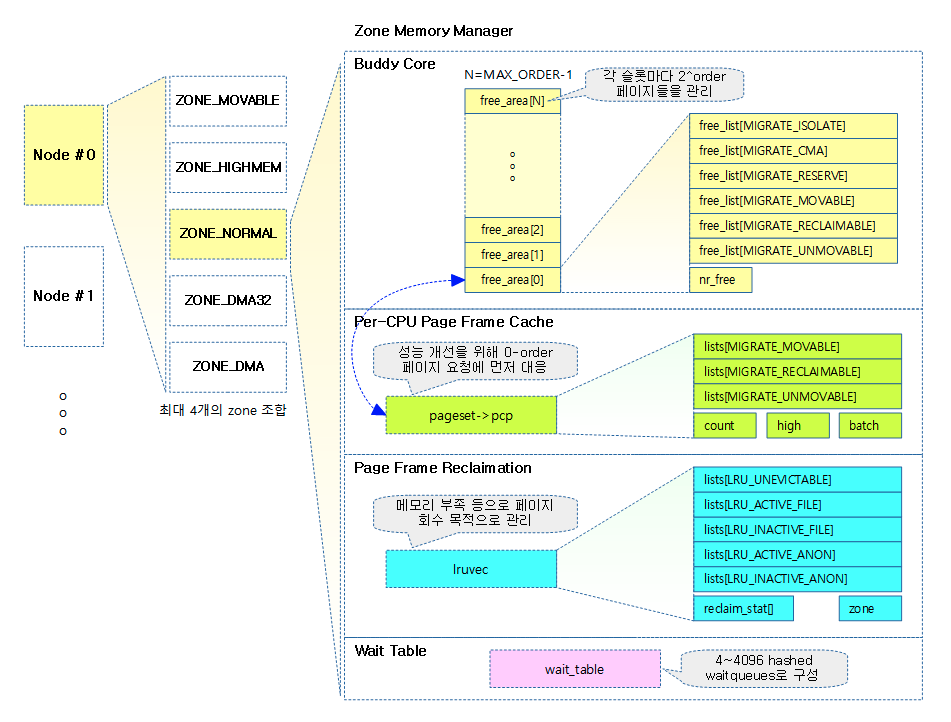
\includegraphics[width=1\textwidth]{figures/zoned_memory.png}
    \caption{Zoned memory allocator}
    \label{fig:zoned_memory_alloc}
\end{figure*}

Our dedicated layered \oursys system. Always allocates elements of 64KB.
This allows to satisfy any allocation needed for network I/O, due to 16 bit used for packet size in IP. For smaller allocations we use the page frag mechanism to allow for a fast, byte granular allocation. We can always assume that small elements allocated together will be freed around the same time. 